\documentclass[8pt,a4paper]{article}
\usepackage{amsfonts}
\usepackage{bbm}
\usepackage{amsmath}
\usepackage{verbatim} 
\usepackage{fullpage}
\usepackage{graphicx}
\usepackage{setspace}
\usepackage{authblk}
\doublespacing

\title{Supplementary file: fecundity model}
\author{}
\date{}
\linespread{1}

\begin{document}
\maketitle
\vspace{-1cm}
We have also analyze a fecundity model.
 In the fecundity model, we assume that the match between the resource use of the species and the type $q$ of a resource unit influences the rate of propagule production but the establishment process is independent of the resource type. 
 Thus, the colonization rate of a resource unit at location $x$ is 
  \begin{equation*}
	r(x,q,n; a, q*,\nu, l, z) = a z^n \left( \sum_{(x' ,q') \in H_O(t)} f_{q*, \nu} (q') D_l(x - x') \right).
\end{equation*}
 where $z \in (0,1]$ controls the severity of the competition and $n$ is the number of other species occupying the resource unit at the time of colonization.
As in the main text, $H_O(t)$ denotes the collection of locations and types of resource units occupied by the focal species  at time $t$ and thus act as propagule sources.
The parameter $a$ is an overall colonization rate parameter and the parameters $q*,\nu , l$ characterize the properties of the species.
$D_{\lambda} (x)$ is top-hat kernel so that $D_l(x) = 1/(\pi l^2)$ if $|x| \leq l$ and $D_l(x) = 0$ if $|x| >  l$. 
The mean field model is
\begin{eqnarray*}
\begin{cases}
\displaystyle{\frac{d}{dt}}\rho(q,t)& = b_R-\mu_R \rho(q,t),\\
\displaystyle{\frac{d}{dt}}\rho_{S}(q,t)& = -\mu_R \rho_S(q,t) -\rho_S(q,t)z^{|S|} \sum_{i \in \mathbb{M} \setminus S} a_i \sum_{J \in S_i} \int_0^1 f_i(q') \rho_J(q',t) dq' \\
 & + \sum_{i \in S} \rho_{S \setminus{\{i\}}}(q,t) z^{|S|-1} a_i \sum_{J \in S_i} \int_0^1 f_i(q') \rho_J(q',t) ds',  \\
\displaystyle{\frac{d}{dt}} \rho_{\mathbb{M}}(q,t) & = - \mu_R \rho_{\mathbb{M}}(q,t) + \sum_{i \in \mathbb{M}} \rho_{\mathbb{M} \setminus{\{i\}}}(q,t) z^{M-1} a_i \sum_{J \in S_i} \int_0^1 f_i(q') \rho_J(q',t) dq'.
\end{cases}
\end{eqnarray*}
%
For the stochastic non-spatial model, the colonization rate for the fecundity model becomes 
\begin{equation*}
r(q, n ; a, q^*, \nu, z) = a z^n \left( \sum_{q' \in H_O(t)} f_{q^*,\nu} (q') \right)\frac{1}{|\Omega|}.
\end{equation*}
Here, $|H_O(t)|$ is the total number of occupied resource units by the focal species at time $t$ and $|\Omega|$ the total area of the landscape.
%
For the deterministic spatial model,  without competition we have  
\begin{eqnarray*}
\begin{cases}
\displaystyle \frac{d}{dt}\rho(x,y,q,t) &= Q(x,y,q) - \mu_R \rho(x,y,q,t), \\
\displaystyle \frac{d}{dt}  \rho_i (x,y,q,t)&=  a_i \left( \rho(x,y,q,t)- \rho_i(x,y,q,t) \right) \int_0^1  f_i(q')(D_i \ast \rho_i) (q') dq' - \mu_R \rho_i(x,y,q,t),
\end{cases}
\end{eqnarray*}
and with competition,
\begin{eqnarray*}
\begin{cases}
\displaystyle \frac{d }{dt} \rho(x,y,q,t) & = Q(x,y,q) - \mu_R \rho(x,y,q,t), \\
\displaystyle \frac{d}{dt}  \rho_i (x,y,q,t) &=  a_i \left( \rho(x,y,q,t)- \sum_{1\leq j \leq M}\rho_j(x,y,q,t) \right) \int_0^1 f_i(q')  (D_i \ast \rho_i) (q') dq' - \mu_R \rho_i(x,y,q,t).
\end{cases}
\end{eqnarray*}

\section{Stability analyzes for the mean field}
\subsection{Mean field fecundity model with only one species}

Ignoring competition between species implies that species dynamics are independent of each other.
Thus, it suffices to study only one species which we indicate by the subscript 1. The set of equations describing the dynamics becomes
\begin{eqnarray*}
\begin{cases}
\displaystyle{\frac{d}{dt}}\rho(q,t) &= b_R-\mu_R \rho(q,t), \\
\displaystyle{\frac{d}{dt}}\rho_1(q,t) &= (\rho(q,t)-\rho_1(q,t)) a_1 \left(\int_0^1  f_1(q') \rho_1(q',t) dq'\right) -\mu_R \rho_1(q,t).
\end{cases}
\end{eqnarray*}
We assume that $b_R$, $\mu_R$ and the initial conditions do not depend on the resource type $q$ in the sense that $\rho(q,0)=\rho(0)$ and $\rho_1(q,0)=\rho_1(0)$. 
It is easy to see that in this case $\rho$ and $\rho_1$ remain independent of $q$ for all times $t$ and thus also for the equilibrium. 
The density of resource units has a unique stable equilibrium: $\displaystyle{ \rho^* = \frac{b_R}{\mu_R}}$. 
There are 2 equilibria for density of occupied resource units by species 1, the trivial equilibrium
\begin{equation}
\rho_1^* = 0
\end{equation}
and the non-trivial equilibrium
\begin{equation}
\rho_1^* = \frac{b_R}{\mu_R}- \frac{\mu_R}{a_1}.
\end{equation}

Let us examine the stablity of the trivial equilibrium $\displaystyle{\rho^* =\frac{b_R}{\mu_R}}$ and $\rho_1 ^* =0$ to ask if the species 1 can invade the system if starting from low density.
Consider the dynamics starting from a small perturbation around this solution, $\rho(q,t)=\rho^*(q)+\epsilon \tilde{v}(q,t)$ and $\rho_1(q,t)=\epsilon \tilde{w}(q,t)$. For small $\epsilon$ we may linearise to obtain
\begin{eqnarray}
\frac{d}{dt} \tilde{v}(q,t) &=& - \mu_R \tilde{v}(q,t), \\
\frac{d}{d t} \tilde{w}(q,t) &=& \frac{b_R a_1}{\mu_R} \left(\int_0^1 f_1(q') \tilde{w}(q',t) dq'\right) -\mu_R \tilde{w}(q,t).
\end{eqnarray}
Assuming that $\tilde{w}(q,t)= w(q) \exp(\lambda t)$ where $w(q)$ is a non-negative function, we get

$$\frac{d}{dt} \tilde{w}(q,t)= \lambda w(q) \exp(\lambda t)= \lambda \tilde{w}(q,t).$$ Hence $\tilde{w}(q,t)$ is an eigenfunction having $\lambda$ as eigenvalue for the operator derivative with respect to time. Replacing $\tilde{w} (q,t)$ by $  w(q) \exp(\lambda t) $  in equation (4) gives

\begin{eqnarray*}
\lambda w(q) \exp(\lambda t)& = & \left(\frac{b_R a_1}{\mu_R} \left(\int_0^1 f_1(q') w(q') dq'\right) -\mu_R w(q)\right) \exp(\lambda t).
\end{eqnarray*}
and thus
$$\lambda w(q) = \frac{b_R a_1}{\mu_R} \int_0^1 f_1(q') w(q') dq' -\mu_R w(q)$$ 
which has the implicit solution
$$w(q) = \frac{b_R a_1}{\mu_R(\lambda +\mu_R )} \int_0^1 f_1(q') w(q')dq'. $$
Multiplying both sides by $f_1(q)$ and then integrating from 0 to 1 w.r.t. $q$, we obtain 
$$1= \frac{b_R a_1}{\mu_R (\lambda+ \mu_R)}.$$
It follows that $\lambda$ is negative if and only if $ b_R a_1 < \mu_R^2.$ Such condition means that the function $\tilde{w}(q,t)$ decays to $0$ exponentially and the system returns to the trivial equilibrium.  
Therefore, the trivial equilibrium is unstable if and only if
\begin{equation}
 a_1 > \frac{\mu_R^2}{b_R}.
\end{equation}
%Assuming that the relation (5) is true, we know that the trivial equilibrium is unstable and since there is only one non-trivial equilibrium (2) %such equilibrium must be stable.

\subsection{ Mean field fecundity model with competition}

To start with, let us assume that there are only two species $1$ and $2$ with respective fitness functions $f_1(q)$ and $f_2(q)$ and colonization rate parameters $a_1$  and $a_2$. We consider the limiting case of extreme competition where $z \rightarrow 0$ and look at conditions allowing coexistence. 
The dynamics of the system are described by the equations
\begin{eqnarray*}
\begin{cases}
 \displaystyle{\frac{d}{dt}}\rho(q,t)&= b_R - \mu_R \rho(q,t),\\
 \displaystyle{\frac{d}{dt}}\rho_1(q,t)&=  (\rho(q,t)-\rho_1(q,t)-\rho_2(q,t)) a_1 \int_0^1 f_1(q) \rho_1(q',t)dq'- \mu_R \rho_1(q,t), \\
 \displaystyle{\frac{d}{dt}}\rho_2(q,t)&=  (\rho(q,t)-\rho_1(q,t)-\rho_2(q,t)) a_2 \int_0^1 f_2(q) \rho_2(q',t)dq'- \mu_R \rho_2(q,t).
 \end{cases}
\end{eqnarray*} 
We approach here the question on coexistence through the mutual invasibility criterion, thus assuming that two species can coexist if each species can invade the other species when the later is at equilibrium. We assume that condition (5) is satisfied for species 1 and that species 1 and the total resource density are at their non-trivial equilibria  $\displaystyle{\rho_1^* = \frac{b_R}{\mu_R}- \frac{\mu_R}{a_1}}$ and $\displaystyle{\rho^*= \frac{b_R}{\mu_R}}$ respectively. To examine under which condition species 2 is able to invade, we consider the following perturbations
\begin{eqnarray*}
 \rho^*(q,t)&= &\rho^*(q)+\epsilon \tilde{v}(q,t), \\
 \rho_1^*(q,t)&= &\rho_1^*(q)+\epsilon \tilde{w_1}(q,t), \\
 \rho_2^*(q,t)&= &\rho_2^*(q)+\epsilon \tilde{w_2}(q,t)=\epsilon \tilde{w_2}(q,t).
\end{eqnarray*} 
Since $\epsilon$  is small we can  linearise and thus have 
\begin{eqnarray*}
\frac{d}{dt} \tilde{v}(q,t) &=& - \mu_R \tilde{v}(q,t),\\
\frac{d}{d t} \tilde{w_1}(q,t) &=& - \mu_R \tilde{w_1} (q,t) +(\rho^*(q)-\rho_1^*(q))a_1 \int_0^1  f_1(q') \tilde{w_1}(q',t) dq' +  \tilde{v}(q,t) a_1  \int_0^1 f_1(q) \rho_1^*(q')dq',\\
\frac{d}{d t} \tilde{w_2}(q,t) &=& (\rho^*(q)-\rho_1^*(q)) a_2\int_0^1  f_2(q') \tilde{w_2}(q',t) dq' - \mu_R \tilde{w_2}(q,t).
\end{eqnarray*}
If there is an eigenfunction $\tilde{w_2}(q,t)= w_2(q) \exp(\lambda t)$ with eigenvalue $\lambda$ where $w_2(q)$ is non-negative, then
\begin{eqnarray*}
\lambda w_2(q)= (\rho^*(q)-\rho_1^*(q))a_2 \int_0^1 f_2(q') w_2(q') dq' - \mu_R w_2(q).
\end{eqnarray*} 
Replacing $\rho^*$ and $\rho_1^*$  by their respective values gives
\begin{eqnarray*}
\lambda w_2(q)= \frac{\mu_R}{a_1}a_2 \int_0^1 f_2(q') w_2(q') dq' - \mu_R w_2(q)
\end{eqnarray*} 
which leads to
\begin{eqnarray*}
 \lambda =  \mu_R (\frac{a_2}{a_1} -1).
\end{eqnarray*} 
 If $\lambda$ is positive, the equilibrium is unstable. Hence, species 2 can invade species 1 if and only if
\begin{eqnarray*}
  a_2 < a_1.
\end{eqnarray*}
As corollary, two (and more species by induction) can coexist if and only if $a_i = a_j$ for all $i, j$. If the species have different colonization rate parameters, only the one with the highest parameter will persist.

\subsection{ Mean field fecundity model with multiple species with the same colonization rate parameter}

Assuming that all species have equal colonization rate parameters, for brevity we denote $a_i = a $ for all $i= 1,\ldots, M$ where $M$ denotes the total number of species. Since the dynamics do not depend on $q$, we also omit the variable $q$ in the notation: $\rho_i(q,t)=\rho_i(t)$ and $\rho(q,t)=\rho(t)$. We have
\begin{eqnarray}
\begin{cases}
\displaystyle{\frac{d}{dt}}\rho(t) &= b_R-\mu_R \rho(t), \\
\displaystyle{\frac{d}{dt}}\rho_i(t) &= a \rho_i(t)  \left(\rho(t)- \sum_{k=1}^M \rho_k(t)\right) -\mu_R \rho_i(t), \;  \forall i \in M.
\end{cases}
\end{eqnarray}
Let $\rho_O(t)= \sum_{k=1}^M \rho_k(t)$ denote the density of occupied resource units. We have

\begin{equation*}
\frac{d}{dt} \rho_O(t)= a\rho_O(t)(\rho(t)-\rho_O(t)) -\mu_R \rho_O(t).
\end{equation*}
The non-trivial equilibrium is $\displaystyle{\rho_O^* = \frac{b_R}{\mu_R}-\frac{\mu_R}{a}}.$ It is easy to see that the density of the occupied resource units at the non-trivial equilibrium is always stable if the non-trivial equilibrium is positive.

Let $\alpha_i >0$ represent the relative densities of the species so that
such that $$\sum_{i=1}^M \alpha_i =1 \mbox{ and } \rho_i^*=\alpha_i \rho_O^*.$$
A simple computation shows that $P^*=  \rho^* \cup \{\rho_i^*\}_{i= 1, \ldots,M}$ is an equilibrium state for the system.  To investigate the stability of this equilibrium, we compute the Jacobian matrix of  the model  (6) evaluated at the equilibrium state $ P^*$.  We obtain

\begin{eqnarray*}
J_{\rho^*\rho^*} &=& \frac{\partial }{\partial \rho } \left( \frac{d}{dt}\rho(t) \right) \bigg|_{P^*}\\
 			& = &  - \mu_R, \\
J_{\rho^* \rho_j^*} &=&  \frac{\partial }{\partial \rho_j } \left( \frac{d}{dt}\rho(t) \right) \bigg|_{P^*}\\
			&=& 0,\\
J_{\rho_i^* \rho^*} &= &  \frac{\partial }{\partial \rho } \left( \frac{d}{dt}\rho_i(t) \right) \bigg|_{P^*}\\ 
			& =& a \rho_i^* \\
			& =&  a \alpha_i \rho_O^*, \\
J_{\rho_i^*\rho_i^*}&=&  \frac{\partial }{\partial \rho_i } \left( \frac{d}{dt}\rho_i(t) \right) \bigg|_{P^*}\\ 
			& = & a \left( \rho^*-\sum_{k=1}^M \rho_k^* -{\rho_i^*}^2\right) -\mu_R \\
			&=& a \left(\rho^*-\rho_O^* - {(\alpha_i \rho_O^*)}^2 \right)- \mu_R, \\
J_{\rho_i^*\rho_j^*}&=&  \frac{\partial }{\partial \rho_j } \left( \frac{d}{dt}\rho_j(t) \right) \bigg|_{P^*}\\
			& = & -a\rho_i^* \rho_j^* \\
			&=& -a \alpha_i \alpha_j {\rho_O^*}^2.
\end{eqnarray*}
The Jacobian matrix then has the following form:
\[ \left( 
\begin{array}{ccccc}
-\mu_R & 0 & 0 & \cdots & 0 \\
- a \alpha_1 \rho_O^* & -a {(\alpha_1 \rho_O^*)}^2 & - a \alpha_1 \alpha_2 {\rho_O^*}^2 & \cdots & -a \alpha_1 \alpha_M {\rho_O^*}^2 \\
- a \alpha_2 \rho_O^* & -a \alpha_2 \alpha_1 {\rho_O^*}^2 & - a {(\alpha_2 \rho_O^*)}^2 & \cdots & -a \alpha_2 \alpha_M {\rho_O^*}^2 \\
\vdots & \vdots &\vdots& \ddots & \vdots \\
- a \alpha_M \rho_O^* & -a \alpha_M \alpha_1 {\rho_O^*}^2 & - a \alpha_M \alpha_1 {\rho_O^*}^2 & \cdots & -a {(\alpha_M\rho_O^*)}^2 
\end{array} 
\right)\] 

For any combination of $\{\alpha_i\}_{i=1,\ldots,M}$, there are always two non-zero eigenvalues with negative real parts. These correspond to the dynamics of total resource units and occupied resource units, whereas the remaining eigenvalues are  zero and they correspond to the relative densities of the species among the occupied resource units. In other words, the total densities of resource units and occupied resource units are stable, but the proportions of individiual species are not stable. In Figure 1, the phase plane is shown for 2 species.

\begin{figure}[!ht]
\begin{center}
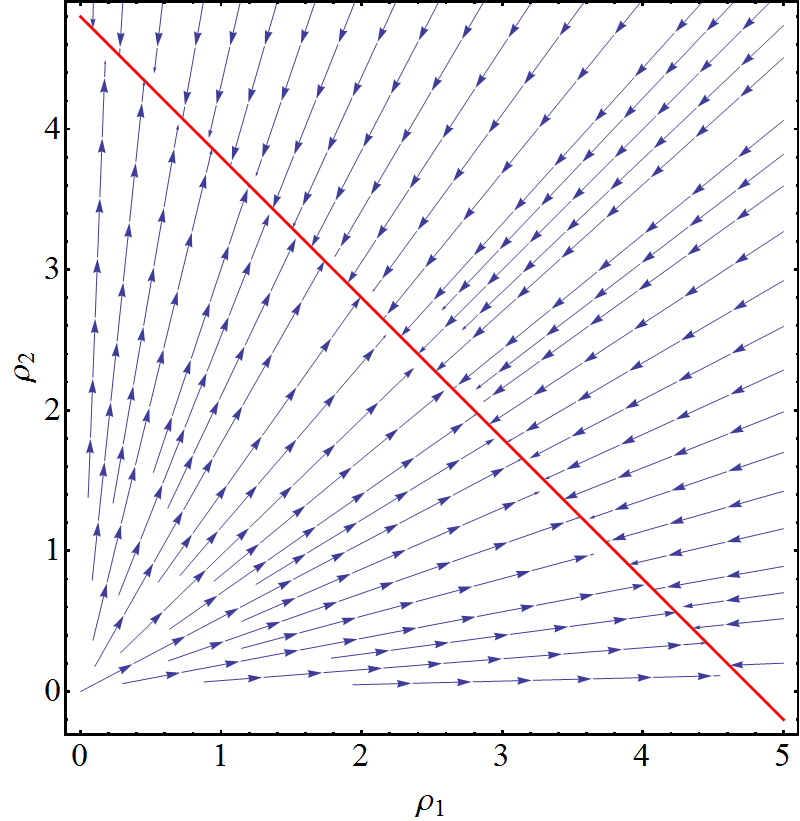
\includegraphics[height=6cm,width=6cm]{FigureX}
\caption{  Phase plane representing the dynamics of the density of resource units occupied by species 1 and 2. Parameters: $a_1= a_2 = 0.5, b_R=0.5, \mu_R= 0.1$.}
\end{center}
\end{figure}

\section{Results from the stochastic models }
Here, we report that the non-monotonic prevalence of the generalist also occurs in the stochastic models.
In the mean field, when the colonization rates of the generalist and the specialist species are equal, the generalist excludes the specialists (thick line in left panels Fig. 2) whereas the specialists exclude the generalists if the former have a higher colonization rate (right panels Fig. 2).
Adding stochasticity generates the hump-shaped pattern in the spatial but also the non-spatial model and thus the results are robust to the part of life-history (fecundity or establishment) in which the species’ specialization influences resource use.

\begin{figure}
\begin{center}
\scalebox{0.65}{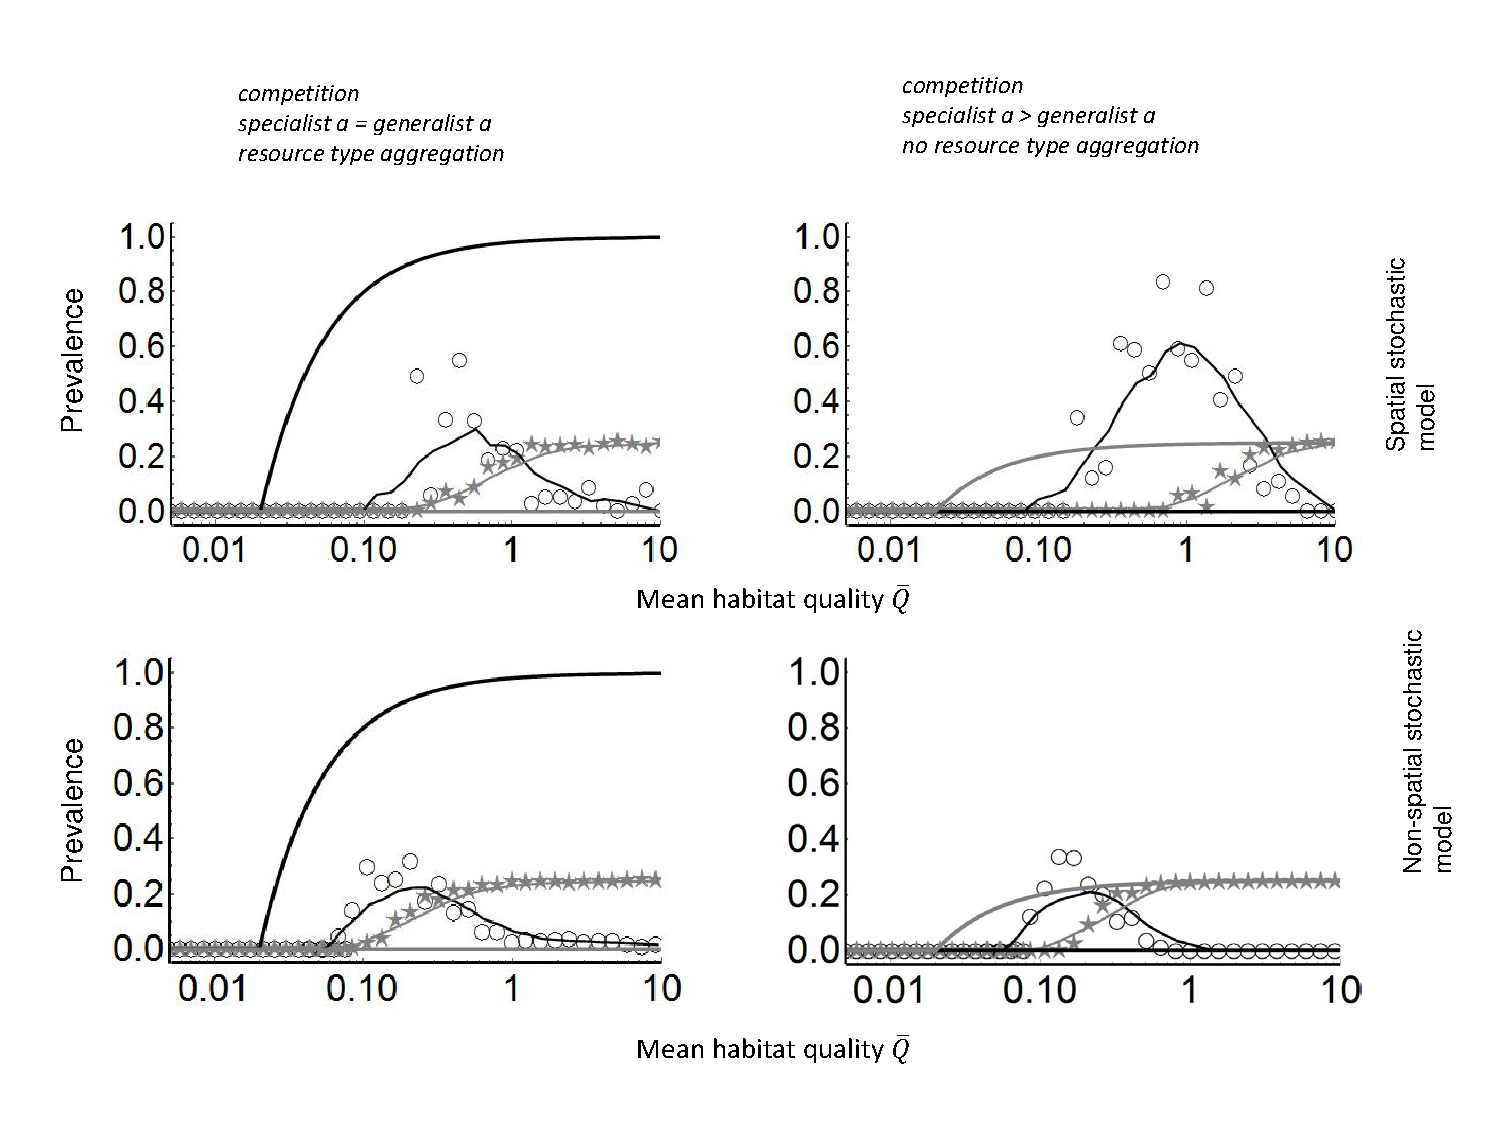
\includegraphics{FigS1}}
\caption{
	Prevalences of a generalist (circles) and specialists (stars) in the spatial and stochastic model (upper row) and non-spatial stochastic model (bottom row).
	The prevalences one generalist species and four highly specialized species ($\nu = 0.125$; shown by solid gray lines in Fig. S1) are shown as function of mean habitat quality 				   $\bar{Q}$ where we varied the resource production rate $\tau$ with fixed $\gamma_H=1$ and $\lambda =0.2$. 
    The colonization rate parameter is $80\%$ lower for the generalist for the left panels. For comparison, the lines show the behavior of the mean-field model. Other parameters as in the main text in  Table 1.
}% Add non trivial units later
\label{FigS1}
\end{center}
\end{figure}



\end{document}


